\subsection{Application Considerations}
\label{sub:application_considerations}

Depending on the operating system, each platform has it's own specific
guidelines on how to provide users with a good experience. Key issues include;
page layout, navigation and interaction.
\marginFig{img/relatedReviews/iOS_page}{iOS page layout recommendation}{fig:iOS_page}

Apple recommends that the most important feature of an app should be displayed
at the top-left of the page so that it will be the first thing a user
sees\cite{HIGApple2013}.  Booking.com and the trainline.com both implement this
well\cite{BookingcomIOS}.
\marginFig[0.8]{img/relatedReviews/booking_page}{Booking page for thetrainline.com\cite{thetrainlineIOS}.}{fig:booking_page}

Users should be able to navigate their way through the app to achieve their
goal of booking sports facilities.

There are 3 main styles of navigation;
\begin{description}
	\item[Hierarchical] navigation is where users make one choice on the first
		screen, another on the second screen and so on until they reach their
		final destination. To navigate to another destination, the user may
		have to retrace some steps or start over from the beginning. This could
		be very inconvenient for the user as they may have to go back several
		steps or start over.
	\item[Content or Experience-driven] navigation depends on the content of
		the application. The navigation also plays an important part of the app
		experience. The Skyscanner app includes a globe,
		figure~\ref{fig:skyscanner_globe}, which allows the user to explore the
		cost of travelling to particular locations. This feature provides a
		unique experience for the user.
		\begin{figure}[htbp]
			\begin{center}
				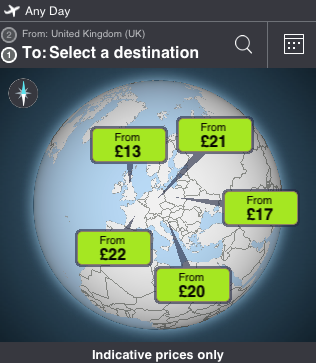
\includegraphics[width=0.4\textwidth]{img/relatedReviews/skyscanner_globe}
			\end{center}
			\caption{Skyscanner apps globe feature}\label{fig:skyscanner_globe}
		\end{figure}

	\item[Flat] navigation allows users to move from one category to another,
		as all categories are available from the main screen. This style has
		been used by many of the apps studied including redspottedhanky.com,
		booking.com and thetrainline.com
		% \begin{figure}[htbp]
		% 	\begin{center}
		% 		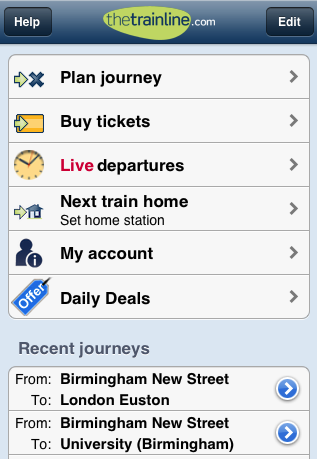
\includegraphics[width=0.25\textwidth]{img/relatedReviews/trainline_main}
		% 	\end{center}
		% 	\caption{Trainline main\cite{thetrainlineIOS}. }\label{fig:trainline_main}
		% \end{figure}
\end{description}

In some cases, it may be better to combine more than one navigation style, but
it could also run the risk of overcomplicating the design of the app and the
user's experience.

Some apps like Trivago have a navigation bar, which manages the screen's
contents. The user can select to change the search criteria or pinpoint hotels
on a map. In the Zipcar app, figure~\ref{fig:zipcar_nav_bar}, the options in
the navigation bar allow the user to perform actions. E.g. `Reserve' or `Log
in'. These options change depending on where the user is in terms of navigation
\begin{figure}[htbp]
	\begin{center}
		
\includegraphics[width=0.45\textwidth]{img/relatedReviews/zipcar_nav_bar1}
		\quad
		
\includegraphics[width=0.45\textwidth]{img/relatedReviews/zipcar_nav_bar2}
	\end{center}
	\caption{Zipcar navigation\cite{ZipCarIOS}.}\label{fig:zipcar_nav_bar}
\end{figure}

Some navigation styles have tab bars placed at the bottom of the screen; this
allows the user to switch between different subtasks, views or modes. For
example, redspottedhanky.com's app includes the options of switching between
finding trains, viewing tickets or account details or finding other
information. This is a useful feature that helps a user navigate their way
through an app, which thetrainline.com has chosen not to use in their design.

Apple and Microsoft both recommend $44\times44$ points and a maximum of 5 icons
to avoid tab bars being over cluttered.
\begin{figure}[htbp]
	\centering
	\begin{subfigure}[b]{0.35\textwidth}
		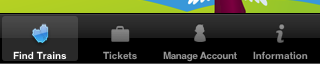
\includegraphics[width=\textwidth]{img/relatedReviews/redspottedhanky_tab_bar}
		\caption{RedspottedHanky tab bar. }\label{fig:redspottedhanky_tab_bar}
	\end{subfigure}%
	\qquad
	\begin{subfigure}[b]{0.4\textwidth}
		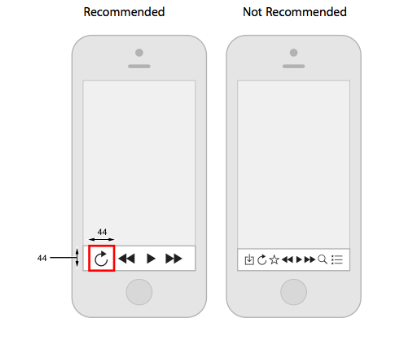
\includegraphics[width=\textwidth]{img/relatedReviews/iOS_tab_bar}
		\caption{iOS tab bar.}\label{fig:iOS_tab_bar}
	\end{subfigure}
	\caption{Tab bar icon sizes.}
\end{figure}

None of the apps studied take into account the orientation of the screen. Users
have no option but to use the apps when the phone is in portrait. It would be
best to provide users with the choice of holding their device in landscape too.
As can be seen in figure~\ref{fig:trivago_input}, Trivago, in particular,
contains a lot of details within its side menu; some users may prefer to see
slightly bigger, which could be possible when the screen is tilted
horizontally.
\marginFig[0.8]{img/relatedReviews/trivago_input}{Trivago input\cite{TrivagoIOS}.}{fig:trivago_input}

The way all of the apps function is through a touchscreen interface. Users may
be used to certain functions such as `pinch to zoom' and other interactions
defined below for iOS\@. It will be important to consider these interactions to
make the app easy to use.
% \begin{figure}[htbp]
% 	\centering
% 	\begin{subfigure}[b]{0.7\textwidth}
% 		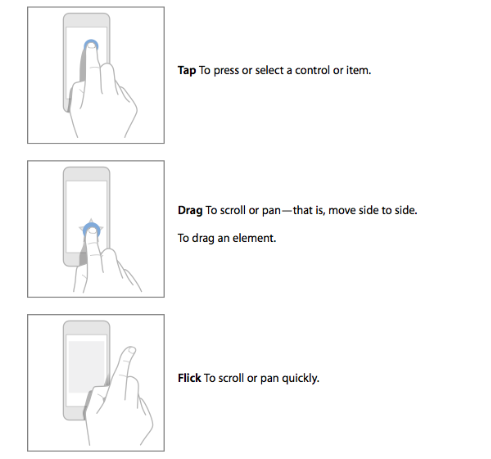
\includegraphics[width=\textwidth]{img/relatedReviews/iOS_touch}
% 		\caption{iOS touchscreen interactions}\label{fig:iOS_touch}
% 	\end{subfigure}%
% 	\qquad
% 	\begin{subfigure}[b]{0.7\textwidth}
% 		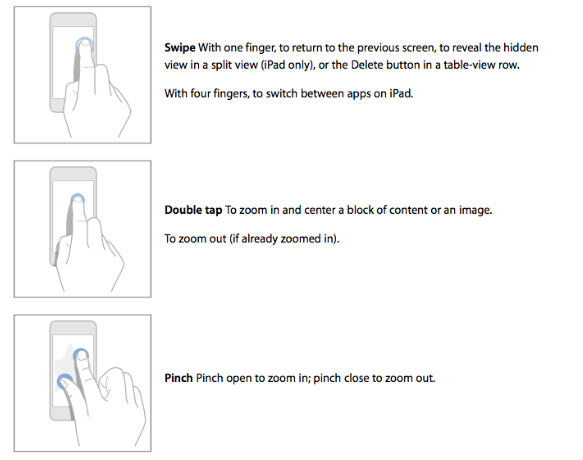
\includegraphics[width=\textwidth]{img/relatedReviews/iOS_touch_2}
% 		\caption{iOS touchscreen interactions}
% 	\end{subfigure}
% 	\caption{}\label{fig:iOS_touch2}
% \end{figure}

Other ways the user could provide input include using speech recognition. For
example, the user could say the sport, date, time and location instead of
having to input text or select options.

% subsection application_considerations (end)
